\section{Formalization of the Run-to-Completion Schedule}
\label{sec:r2c}
Similar to the previous section, the formalization is done using an \EventB context to capture the syntactic elements (Section~\ref{sec:r2c-syntax}) and an \EventB machine to model the semantics (Section~\ref{sec:r2c-semantics}).

\subsection{Formalization of the Run-to-completion Syntactic Elements}
\label{sec:r2c-syntax}
To define run to completion execution we first specify the  syntactic elements involved. 
Triggers, are partitioned into either  Internal or External triggers.
%\begin{center}
%    \EventBInline{partition (TRIGGERS, InternalTriggersType, ExternalTriggerType, {nullTrigger})}
%\end{center}
We define the internal and external trigger queues as sequences of internal and external triggers respectively. Sequences and their allowed operations (e.g. append trigger, head of sequence) are constructively defined via a series of theorems and axioms which are omitted here.

%A null trigger |nullTrigger| is introduced for convenience to simplify the 
%definition of the initial condition. As shown in 
%Figure~\ref{fig:run-to-completion} shows the execution begins by taking untriggered steps which is otherwise only done after a trigger is consumed. Hence the |nullTrigger| is said to be consumed during initialization.
Figure~\ref{fig:run-to-completion} shows the state machine for the run-to-completion schedule. 
From the \emph{Ready to de-queue} state, an internal or (if internal queue empty) external trigger is de-queued from the corresponding queues and the system moves to the \emph{Firing Triggered} state.
A trigger step that consumes the dequeued trigger is then fired and the system moves to the \emph{Firing Untriggered} state. 
From this state, untriggered steps can be fired repeatedly or the system moves back to the \emph{Ready to de-queue} state. 
Both triggered and untriggered steps can raise more internal triggers, which will need to be handled in the future runs.
\begin{figure}[!t]
\centering
\includegraphics[width=0.7\textwidth]{figures/run-to-completion.png}
\caption{State diagram for run to completion scheduling}
\label{fig:run-to-completion}
\end{figure}

The context defining the syntactic elements for a run to completion is shown in Listing~\ref{lst:r2c_ctx}. 
An important notion for the run to completion schedule are steps.  
A triggered  step is taken when an internal or external trigger is consumed and a non-deterministic number of untriggered steps may be taken after a triggered step. 
In the next section we will show how these steps relate to triggered and untriggered transitions  

\begin{lstlisting}[language=Event-B, caption = {Context for Run-to-Completion Semantics}, label = {lst:r2c_ctx}]
context r2c_ctx
extends r2c_c0_2_dequeue 
sets Steps
constants InternalTriggers ExternalTriggers Triggers StepTrigger StepRaised
axioms
	@typeof_IT: InternalTriggers ⊆ InternalTriggerType
	@typeof_XT: ExternalTriggers ⊆ ExternalTriggerType
	@def_T: Triggers = InternalTriggers ∪ ExternalTriggers
	@typeof_StepTrigger: StepTrigger ∈ Steps ⇸ Triggers
	@typeof_StepRaised: StepRaised ∈ Steps → Seq(InternalTriggers)
end
\end{lstlisting} 
Here |StepTrigger| (as a partial function) defines the required trigger for a Step (if any), and |StepRaised| defines the sequence of internal triggers that will be raised for a step (including an empty sequence). Steps that do not have any required trigger will be untriggered steps.

\subsection{Formalization of the Run-to-Completion Semantics}
\label{sec:r2c-semantics}
Given the syntactic elements defined earlier, the machine defining the semantics for the run-to-completion schedule models the trigger queues in the system according to Figure~\ref{fig:run-to-completion}. The dynamic status of the run-to-completion schedule is represented by the variables |int_q|, |ext_q|, |dt| (dequeue trigger), and |completion| with the following invariants.
\begin{EventBcode}
	@int_q: int_q ∈ Seq(InternalTriggers)
	@ext_q: ext_q ∈ Seq(ExternalTriggers)
	@dequeue_trigger: dt ∈ DeQueueType
	@dequeue_triggerwd:	dt ⊆ InternalTriggers ∪ ExternalTriggers
	@firingTriggered: dt ≠ ∅ ⇒ completed=FALSE
\end{EventBcode}
Where |int_q| and |ext_q| represent the sequences of internal and external triggers that need to be handled, |dt| keeps track of the trigger that has been removed from the queues (de-queue) to be consumed by a |TriggeredStep|. Note that |dt| is a singleton set of trigger when the system is in the \emph{Firing Triggered} state and empty otherwise (this is also the definition of |DeQueueType|). Finally, variable |complete| (denoted as |UC| in Figure~\ref{fig:run-to-completion}) is |TRUE| indicates that the system is in the \emph{Ready to de-queue} state.

Starting from the \emph{Ready to de-queue} state (where |completed = TRUE|), the system will de-queue an internal/external trigger if there are any. Note that an external trigger is only de-queued when the internal queue is empty. After that the system moves to the \emph{Firing triggered} state (where |completed = FALSE| and |dt| is no longer empty).
\begin{center}
\begin{minipage}[t]{0.48\textwidth}
\begin{EventBcode}
event dequeueInternalTrigger
any trigger where 
	@grd1: completed = TRUE
	@grd2: int_q ≠ ∅
	@grd3: trigger = Seq_head(int_q)
then 
	@act1: dt ≔ {trigger}
	@act2: int_q ≔ Seq_tail(int_q) 
	@act3: completed ≔ FALSE
end
\end{EventBcode}
\end{minipage}
\hfill
\begin{minipage}[t]{0.48\textwidth}
\begin{EventBcode}
event dequeueExternalTrigger
any trigger where 
    @grd1: completed = TRUE
    @grd2: ext_q ≠ ∅
    @grd3: trigger = Seq_head(ext_q)
    @grd4: int_q = ∅
then 
    @act1: dt ≔ {trigger}
    @act2: ext_q ≔ Seq_tail(ext_q)
    @act3: completed ≔ FALSE
end
\end{EventBcode}
\end{minipage}
\end{center}

The behaviour of the \emph{TriggeredStep} and \emph{UntriggeredStep} are formalised by the corresponding events as follows. Both events can raise a sequence of internal triggers which is concatenated to the the internal queue.
\begin{center}
    \begin{minipage}[t]{0.48\textwidth}
\begin{EventBcode}
event triggeredStep 
any Step where 
    @grd1: Step ∈ dom(StepTrigger)		
    @grd2: StepTrigger(Step) ∈ dt
then 
    @act1: dt ≔ dt ∖ {StepTrigger(Step)}
    @act2: int_q ≔ Seq_concat(int_q ↦ StepRaised(Step))
end
\end{EventBcode}
    \end{minipage}
    \hfill
    \begin{minipage}[t]{0.51\textwidth}
\begin{EventBcode}
event untriggeredStep 
any Step where 
    @grd1: Step ∈ Steps ∖ dom(StepTrigger)	
    @grd2: dt = ∅
then 
	@act1: int_q ≔ Seq_concat(int_q ↦ StepRaised(Step))
end
\end{EventBcode}
    \end{minipage}
\end{center}
While the internal triggers are raised through steps, external triggers can be raised non-deterministically by event |raiseExternalTrigger| and appended to the external queue. 
%Finally, the system can complete when there are no dequeue trigger. 
Note that at this stage (without the statemachine), there is a non-determinism between |untriggeredStep| and |completion|. 
When we combine the untriggered statechart and the run-to-completion schedule in the next section, we will distinguish the two cases.
\begin{center}
    \begin{minipage}[t]{0.55\textwidth}
\begin{EventBcode}
event raiseExternalTrigger
any trigger where
    @grd1: trigger ∈ ExternalTriggers
then
    @act1: ext_q ≔ Seq_append(ext_q ↦ trigger)
end
\end{EventBcode}
    \end{minipage}
    \hfill
    \begin{minipage}[t]{0.43\textwidth}
\begin{EventBcode}
event completion
where
    @grd1: dt = ∅
    @grd2: completed = FALSE
then
    @act1: completed ≔ TRUE
end
\end{EventBcode}
    \end{minipage}
\end{center}

The model of the run-to-completion schedule maintains its invariants straightforwardly (relying on operations of sequence manipulation).